\documentclass{article}
\author{QianLiu}
\date{\today}
\title{Insert Graphic}


%refer to packages
\usepackage{graphicx}
\graphicspath{{figures/}}
\usepackage{ctex}

\begin{document}
    \tableofcontents
    \maketitle
    \section{Insert Graphic}
    \LaTeX{ }the iconograph in article

    \subsection{Insert the picture into \textbackslash being\{figure\}..\textbackslash end\{figure\}}
        \subsubsection{option:[scale=0.3]}
        refer picture \ref{pic_1}
        \begin{figure}[htbp]
            \centering
            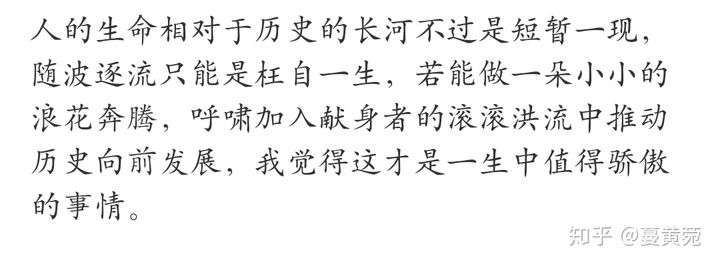
\includegraphics[scale=0.3]{huadanian}
            \caption{黄大年语录}
            \label{pic_1}
        \end{figure}
        
        \subsubsection{option:[width=2cm]}
        refer picture \ref{pic_2}
        \begin{figure}
            \centering
            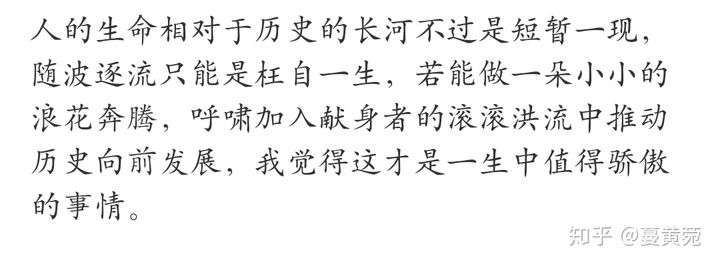
\includegraphics[width=2cm]{huadanian.jpg}
            \caption{黄大年语录}
            \label{pic_2}
        \end{figure}

        \subsubsection{Specify the relative width:[0.5\textbackslash textwidth]}
        \begin{figure}[htbp]
            \centering
            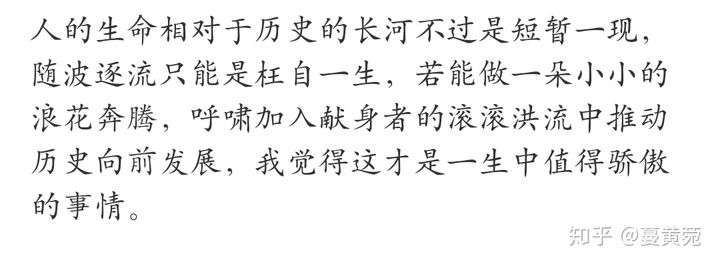
\includegraphics[width=0.5\textwidth]{huadanian.jpg}
            \caption{黄大年语录}
        \end{figure}

    \section{Insert table}
        \subsection{Insert table in \textbackslash being\{table\}...\textbackslash end\{table\}}
        \begin{table}[htbp]
            \centering
            \caption{The \ref{tab_1} table}
            \begin{tabular}{|c|c|}
                \hline
                name & age \\
                \hline\hline
                QianLiu & 23 \\
                \hline
            \end{tabular}
            \label{tab_1}% Notice the position of \label
        \end{table}
\end{document}